\documentclass{article}

\usepackage{graphicx}
\usepackage{tikz}
\usepackage{tikzsymbols}
\usetikzlibrary{calc,patterns,shapes.geometric}
\pagestyle{empty}
\usepackage[margin=0pt]{geometry}
\geometry{papersize={14in,12in}}

\def\centerarc[#1](#2)(#3:#4:#5){\draw[#1] ($(#2)+({#5*cos(#3)},{#5*sin(#3)})$) arc (#3:#4:#5);}

\begin{document}
	\begin{figure}
		\centering
		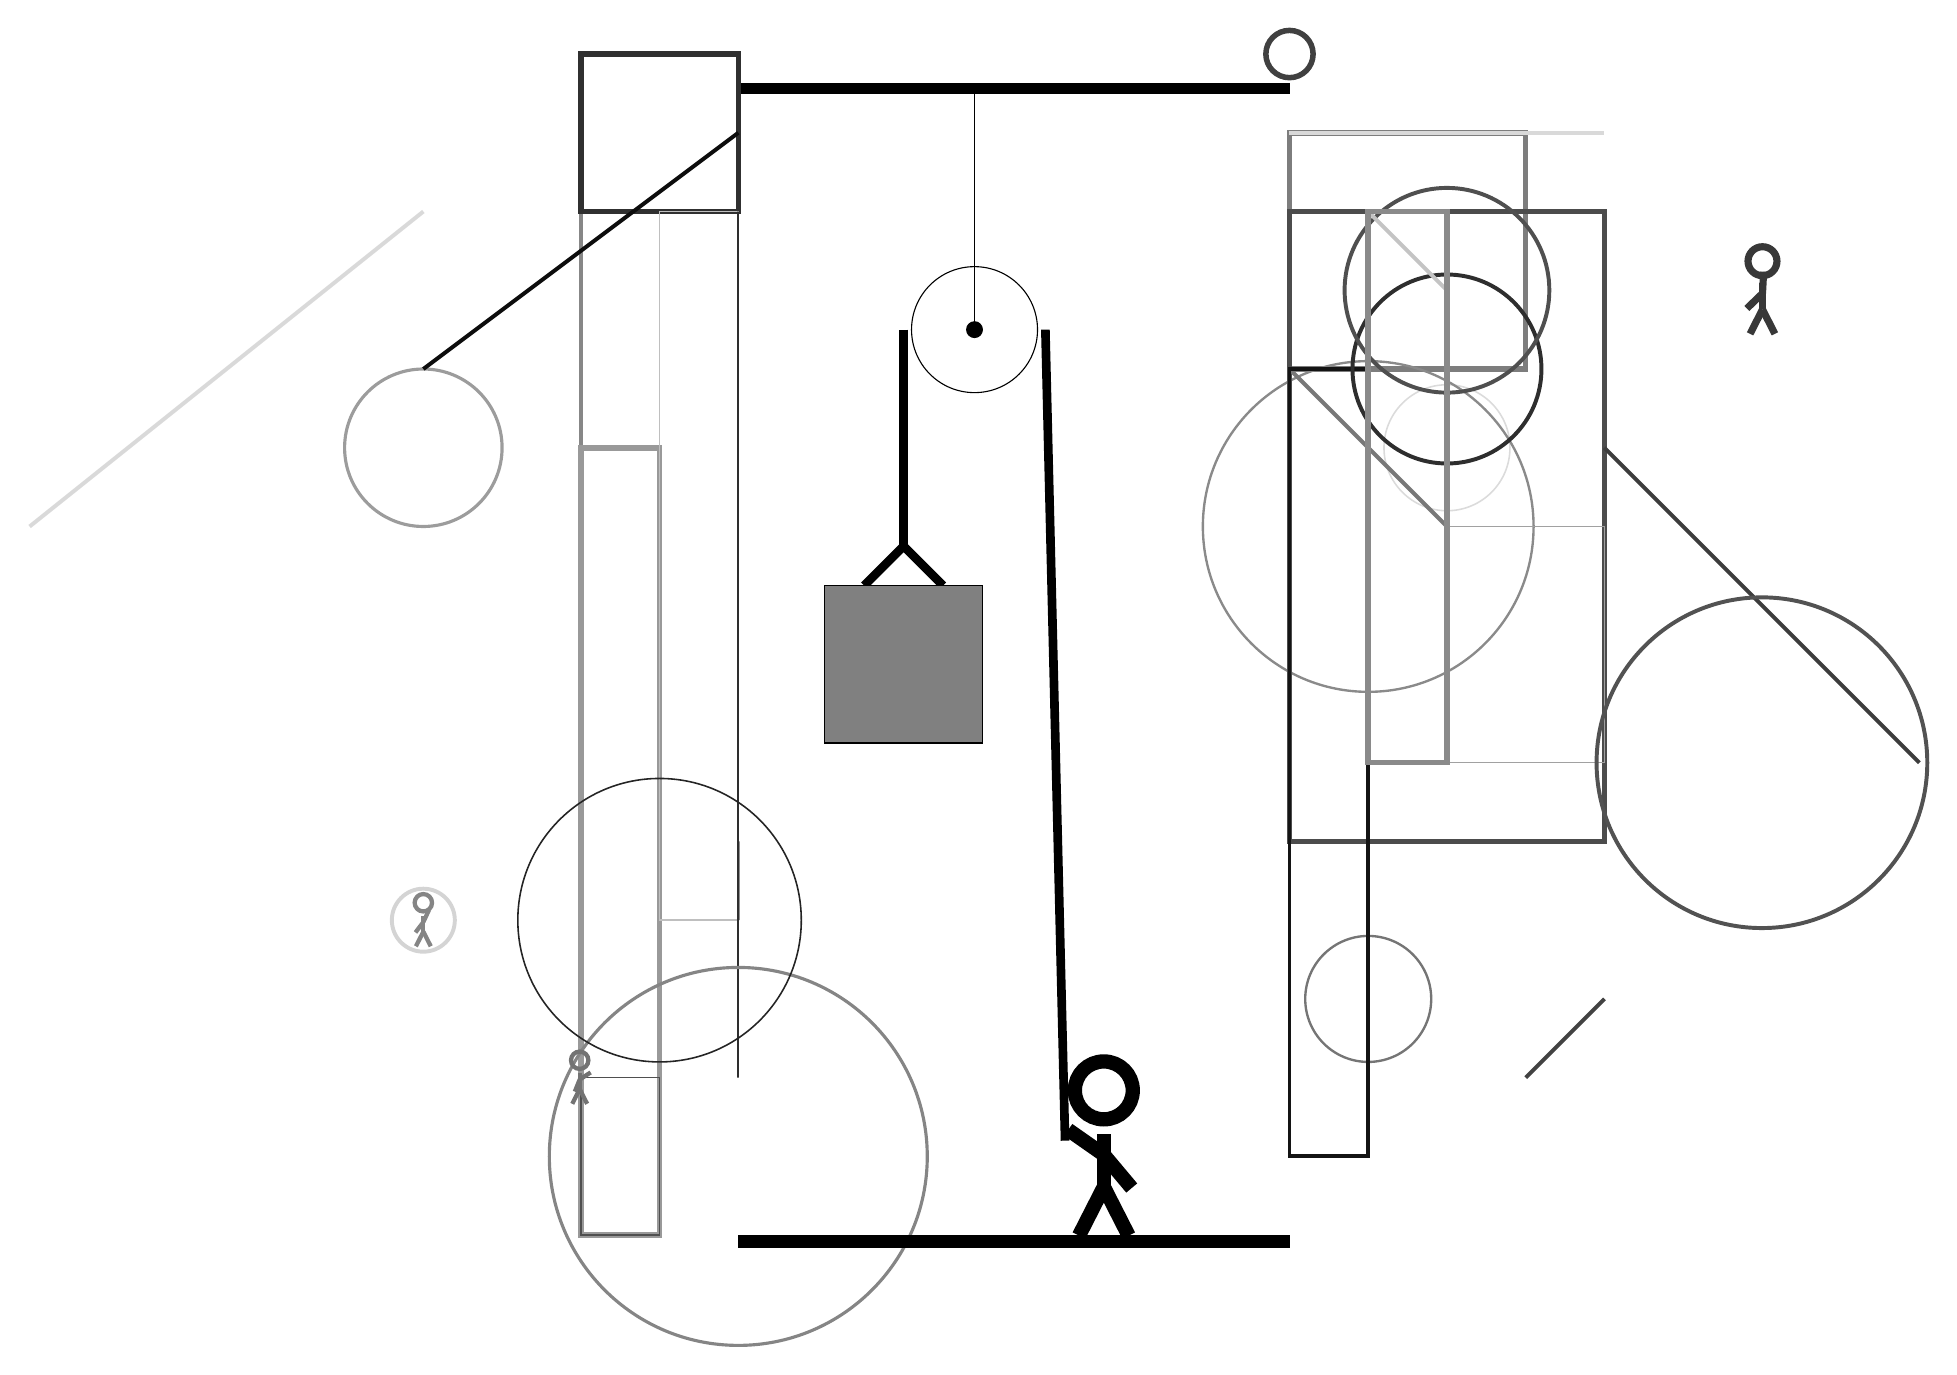
\begin{tikzpicture}
			%%%%% START %%%%%
			
			\draw[fill=black] (-2, 11.5) rectangle (5, 11.625);
			
			\draw (1, 8.5) circle (0.8);
			\draw[fill=black] (1, 8.5) circle (0.1);
			\draw (1, 11.5) -- (1, 8.5);
			
			\draw[line width=1.1mm] (-0.4, 5.25) -- (0.1, 5.75) -- (0.6, 5.25);
			\draw[fill=black!50] (-0.9, 5.25) rectangle (1.1, 3.25);
			
			\draw[line width=1.1mm] (0.1, 8.5) -- (0.1, 5.75);
			\centerarc[line width=1.1mm](1, 8.5)(0:180:0.9);
			\draw[line width=1.1mm](1.9, 8.5) -- (2.15, -1.8);
			
			\node at (2.6, -1.9) {\Strichmaxerl[10][-35][-50]};
			
			\draw [line width=0.4mm, color=black!39](-6, 7) circle (1.0);
			
			\draw[line width=0.7mm, color=black!51] (5, 8) rectangle (8, 11);
			\draw [line width=0.2mm, color=black!14](7, 7) circle (0.8);
			\draw [line width=0.3mm, color=black!46](6, 6) circle (2.1);
			\draw[line width=0.7mm, color=black!70] (5, 10) rectangle (9, 2);
			
			\draw[line width=0.5mm, color=black!47](-4, -2) -- (-4, 12);
			
			\node[line width=0.2mm, color=black!78] at (11, 9) {\Strichmaxerl[5][44][87]};
			
			\draw [line width=0.5mm, color=black!17](-6, 1) circle (0.4);
			\draw[line width=0.4mm, color=black!44] (-2, 1) rectangle (-2, 2);
			\draw[line width=0.5mm, color=black!53](7, 6) -- (5, 8);
			\draw [line width=0.3mm, color=black!54](6, 0) circle (0.8);
			\draw[line width=0.7mm, color=black!81] (-4, 12) rectangle (-2, 10);
			\draw[line width=0.5mm, color=black!92] (5, -2) rectangle (6, 8);
			
			\draw[line width=0.7mm, color=black!40] (-4, 7) rectangle (-3, -3);
			\draw[line width=0.2mm, color=black!69] (-4, -1) rectangle (-3, -3);
			\node[line width=0.6mm, color=black!48] at (-6, 1) {\Strichmaxerl[3][53][65]};
			
			\draw [line width=0.5mm, color=black!82](7, 8) circle (1.2);
			\draw[line width=0.5mm, color=black!95](-6, 8) -- (-2, 11);
			\draw[line width=0.5mm, color=black!15](-6, 10) -- (-11, 6);
			\draw[line width=0.2mm, color=black!25] (-2, 1) rectangle (-3, 10);
			\draw[line width=0.3mm, color=black!82] (-2, 10) rectangle (-2, -1);
			
			\draw [line width=0.4mm, color=black!48](-2, -2) circle (2.4);
			
			\draw [line width=0.2mm, color=black!86](-3, 1) circle (1.8);
			\draw [line width=0.5mm, color=black!69](7, 9) circle (1.3);
			\draw[line width=0.5mm, color=black!76](9, 7) -- (13, 3);
			\draw[line width=0.5mm, color=black!23](6, 10) -- (7, 9);
			\draw[line width=0.2mm, color=black!37] (7, 3) rectangle (9, 6);
			\draw [line width=0.5mm, color=black!68](11, 3) circle (2.1);
			
			\draw[line width=0.5mm, color=black!15](5, 11) -- (9, 11);
			\draw [line width=0.7mm, color=black!75](5, 12) circle (0.3);
			\node[line width=0.7mm, color=black!55] at (-4, -1) {\Strichmaxerl[3][68][33]};
			
			\draw[line width=0.7mm, color=black!46] (6, 10) rectangle (7, 3);
			\draw[line width=0.5mm, color=black!74](8, -1) -- (9, 0);
			
			\draw[fill=black] (-2, -3) rectangle (5, -3.15);
			
			%%%%% END %%%%%
		\end{tikzpicture}
	\end{figure}	
\end{document}